\documentclass[10pt,a4paper]{article}

\usepackage[utf8]{inputenc}		% Configuro la codificación
\input{.command.tex}
% En el siguiente archivo se configuran las variables del trabajo práctico
%% \providecommand es similar a \newcommnad, salvo que el primero ante un 
%% conflicto en la compilación, es ignorado.

% Al comienzo de un TP se debe modificar los argumentos de los comandos


\providecommand{\myTitle}{TRABAJO PRÁCTICO Nº2}
\providecommand{\mySubtitle}{Radiación}

\providecommand{\mySubject}{Electromagnestismo (82.06)}
\providecommand{\myKeywords}{UBA, Ingeniería, Informe, semiconductor}

\providecommand{\myAuthorSurname}{Alacaraz, Manso & Zuccolo}
\providecommand{\myTimePeriod}{Año 2018 - 1\textsuperscript{er} Cuatrimestre}

% No es necesario modificar este %%%%%%%%%%%%%%
\providecommand{\myHeaderLogo}{header_fiuba}
%%%%%%%%%%%%%%%%%%%%%%%%%%%%%%%%%%%%%%%%%%%%%%%%

% Si se utilizan listings, definir el lenguaje aquí
\providecommand{\myLanguage}{matlab}

% Crear los integrantes del TP con el comando \PutMember donde
%%		1) Apellido, Nombre
%%		2) Número de Padrón
%%		3) E-Mail
\providecommand{\MembersOnCover}[0]
{		\PutMember{Alcaraz, Gonzalo} {93874} {g.alcaraz@outlook.com}
		\PutMember{Manso, Juan} {96133} {juanmanso@gmail.com}
		\PutMember{Zuccolo, Florencia} {96628} {florenciaz618@gmail.com}
}

\providecommand{\myGroupNumber}{16}

\Pagebreaktrue		% Setea si hay un salto de página en la carátula
\Indextrue
\Siunitxtrue			% Si quiero utilizar el paquete, \siunixtrue. Si no \siunixfalse
\Todonotestrue		% Habilita/Deshabilita las To-Do Notes y las funciones \unsure, \change, \info, \improvement y \thiswillnotshow.
\Listingsfalse
\Keywordsfalse
\Putgrouptrue		% Habilita/Deshabilita el \myGroup en los headers
\Videofalse
				% Archivo con los comandos globales como Título y autores
%Preambulo para articulo científico de LaTeX

\usepackage[a4paper,left=3cm,right=3cm,bottom=3.5cm,top=3.5cm]{geometry} 	% Configuro la geometría del papel
%\usepackage{microtype}								% Mejora el "spacing" de las palabras
\usepackage[spanish]{babel} 							% Compatibilizo los signos del español
	\addto\captionsspanish{\renewcommand{\tablename}{Tabla}}		%% Redefino nombres preestablecidos por Babel
	\addto\captionsspanish{\renewcommand{\listtablename}{Índice de tablas}}	%% y así en vez de Cuadro dirá Tabla.
\usepackage{amsmath, amsfonts, amssymb}						% Entornos matemáticos, fuentes y símbolos
\usepackage{graphicx}								% Necesario para insertar figuras
\usepackage{fancyhdr}								% Para manipular headers y footers
\usepackage[usenames,dvipsnames]{color}						% \color{color deseado} {lo que querés que tenga color}
\usepackage{subcaption}								% Permite captions del tipo 1a, 1b
\usepackage{multirow}								% Para tablas
\usepackage{float}

% Para video
\ifVideo
	\usepackage{media9}
	\addmediapath{./../reportes/}
\fi

%\usepackage{times}
%\usepackage{mathtools}
\usepackage{upgreek} % letras griegas sin cursiva
%\usepackage{cancel}
\usepackage{rotating}
\usepackage{tikz}
\usepackage{pgfplots}
%	\pgfplotsset{compat=1.12}
	\usetikzlibrary{plotmarks}% matlab2tikz
\usepackage{grffile}% matlab2tikz 
	\usetikzlibrary{calc,patterns,decorations.pathmorphing,decorations.markings}

\ifListings
	\usepackage{listings}

	\providecommand{\lstinputpath}[1]{\lstset{inputpath=#1}}

	\input{.lst_default.tex}
%	\input{.lst_matlab.tex}
%	\input{.lst_c.tex}
%	\input{.lst_c++.tex}
	
% 	\input{.lst_pseudocode.tex}


\fi

\ifSiunitx
\usepackage{siunitx}											% Unidades: \SI {cantidad} {\unidad} (necesita texlive-science)
	\sisetup{load-configurations = abbreviations}							% Habilita poner \cm en vez de \centi\metre
	\sisetup{output-decimal-marker = {,}}									% Cambia los puntos decimales por comas
	\sisetup{per-mode = fraction}											% Pone las unidades como fracción
	\sisetup{quotient-mode = fraction}										
\fi

\ifTodonotes
\usepackage{xargs}
\usepackage[colorinlistoftodos,prependcaption,textsize=tiny]{todonotes}


	\newcommandx{\Juan}[2][1=]{\todo[linecolor=red,backgroundcolor=red!25,bordercolor=red,#1]{#2}}
	\newcommandx{\Gonza}[2][1=]{\todo[linecolor=blue,backgroundcolor=blue!25,bordercolor=blue,#1]{#2}}
	\newcommandx{\Flor}[2][1=]{\todo[linecolor=OliveGreen,backgroundcolor=OliveGreen!25,bordercolor=OliveGreen,#1]{#2}}
	\newcommandx{\improvement}[2][1=]{\todo[linecolor=Plum,backgroundcolor=Plum!25,bordercolor=Plum,#1]{#2}}
	\newcommandx{\thiswillnotshow}[2][1=]{\todo[disable,#1]{#2}}
\fi

\usepackage{booktabs}														% Permite hacer tablas sin separadores en el medio
\usepackage{placeins}														
		\let\Oldsection\section												%% Permite que los flotantes (como figuras) no aparescan
	\renewcommand{\section}{\FloatBarrier\Oldsection}						%% antes o después de su sección correspondiente.
		\let\Oldsubsection\subsection
	\renewcommand{\subsection}{\FloatBarrier\Oldsubsection}		
		\let\Oldsubsubsection\subsubsection
	\renewcommand{\subsubsection}{\FloatBarrier\Oldsubsubsection}
\usepackage{hyperref}														% Debe ser agregado al final del preambulo

\hypersetup
{    bookmarks=true,         % show bookmarks bar?
     unicode=false,          % non-Latin characters in Acrobat’s bookmarks
     pdftoolbar=true,        % show Acrobat’s toolbar?
     pdfmenubar=true,        % show Acrobat’s menu?
     pdffitwindow=false,     % window fit to page when opened
     pdftitle={\myTitle},    		 % title
     pdfauthor={\myAuthorSurname},   % author
	 pdfcreator={\myAuthorSurname},	 % creator = author
     pdfsubject={\mySubject},		 % subject of the document
     pdfkeywords={\myKeywords},
     colorlinks=true,        % false: boxed links; true: colored links
     linkcolor=black,        % color of internal links (change box color with linkbordercolor)
     citecolor=black,        % color of links to bibliography
     filecolor=magenta,      % color of file links
     urlcolor=cyan           % color of external links
}

%Configuro la pagina con los encabezaos y pies de paginas
\pagestyle{fancy}										% Para agregar encabezados y pie de paginas	
\lhead{\mySubject}										% Encabezado izquierdo
\rhead{\includegraphics[scale=0.15]{\myHeaderLogo}} 	% Encabezado derecho (logo de la FIUBA)	
\ifPutgroup
\chead{\texttt{Grupo Nº\myGroupNumber} \\ \textit{\footnotesize{\myTimePeriod}}}
\fi				


% Defino el path de los includegraphics
\graphicspath{{./Figuras/}{./imagenes/}}		% Directorio que contiene los graficos

% Defino el path para los input de .tex y de .eps
\makeatletter
\def\input@path{{./Figuras/}{./Secciones/}{./Cover_page/}{./imagenes}{./Tikz}}
\makeatother

% Defino el path del listings
\ifListings
%% Cambiar el nombre de la carpeta si se utilizan Listings
	\lstinputpath{../Secciones}
\fi


\begin{document}
		% Carátula (formal o simple,_formal o _simple respectivamente),
		% Resumen e Índice (si es necesario configurar en config.tex) del informe
		\begin{titlepage}
	
		\thispagestyle{empty}

		\begin{center}
			
\includegraphics[scale=0.3]{fiuba}\\
			\large{\textsc{Universidad de Buenos Aires}}\\
			\large{\textsc{Facultad De Ingeniería}}\\
			\small{\myTimePeriod}
		\end{center}

		\vfill

		\begin{center}
			\Large{\underline{\textsc{\mySubject}}}
		\end{center}

		\vfill

		\begin{tabbing}
			\hspace{2cm}\=\+\myTitle\\
				TEMA: \mySubtitle\\
				FECHA: \today\\
				\ifPutgroup
					GRUPO: \myGroupNumber\\
				\fi

			\\
				\MembersHeader
				\MembersOnCover	
		\end{tabbing}

		\begin{abstract}
			El presente trabajo práctico tiene como objetivo modelizar y analizar cierta configuración de radiadores en el entorno de altas frecuencias. Para ello se utiliza el \textit{software} numérico \textit{4nec2}. Por otra parte, se diseña un adaptador de impedancias mediante el uso de la Carta de Smith.
		\end{abstract}

	\ifKeywords
		\begin{center}
			\emph{Palabras Clave: \myKeywords}
		\end{center}
	\fi	

		\vfill
	
\end{titlepage}

\ifPagebreak
	\thispagestyle{empty}
	\ifIndex
		\tableofcontents
%		\listoffigures
%		\listoftables
	\fi

	\pagebreak
\fi


	\setcounter{page}{1}
	\section{Desarrollo}
		\input{desarrollo.tex}
		\subsection{Método de momentos}
			\begin{equation}
	\centering
	V_m = \sum_{n=1}^N Z_{nm} I_m
\end{equation}

\begin{equation}
	\centering
	V_m = -j\omega \epsilon \int_{C(\bold{r})} E^i (\bold{r}) f_m(\bold{r}) d\bold{r}
\end{equation}	

\begin{equation}
	\centering
	Z_{nm} = \int_{C(\bold{r})} \int_{C(\bold{r'})} f_n(\bold{r'})\left[ \left(\frac{\partial^2}{\partial{z^2}} + \beta ^2 \right) G(\bold{r},\bold{r'}) \right] f_m(\bold{r}) d\bold{r'} d\bold{r}
\end{equation}


El método de momentos de la radiación se basa en la implementación de la ecuación de Pocklington. Para analizar la radiación de antenas, se divide la estructura metálica en elementos radiantes. Uno de estos elementos se conecta a una fuente de energía que se modela como fuente de tensión concentrada $V_m$. A partir de la resolución de un sistema lineal se obtiene la corriente de cada elemento que compone la estructura para una determinada frecuencia. Una vez obtenida la ditribución de corriente, se calcula el potencial vectorial \eqref{ec.A} y los campos eléctricos \eqref{ec.E} y magnéticos \eqref{ec.E} raidados por la estructura.

El software \textit{4nec2} permite resolver numéricamente las ecuaciones que describen la forma de la distribución de corriente ya sea proveniente de una fuente ó por inducción.

\begin{equation}
	\centering
	\bold{A} = \frac{\mu}{4 \cdot \pi} \int_{C(\bold{r'})} I(\bold{r'}) \frac{ \exp{(-i\beta R)} }{R} \bold{\hat{I}} dl'
	\label{ec.A}
\end{equation}	

\begin{equation}
	\centering
	\bold{E} = \frac{\nabla \times \bold{H} }{ j\omega\epsilon}
	\label{ec.E}
\end{equation}	

\begin{equation}
	\centering
	\bold{H} = \frac{\nabla \times \bold{H}}{j\omega \epsilon}
	\label{ec.H}
\end{equation}

	
		\subsection{Geometría a simular}
			\begin{figure}[H]
	\centering
	\scalebox{0.7}{% XCircuit output "config6.tex" for LaTeX input from config6.ps
\def\putbox#1#2#3#4{\makebox[0in][l]{\makebox[#1][l]{}\raisebox{\baselineskip}[0in][0in]{\raisebox{#2}[0in][0in]{\scalebox{#3}{#4}}}}}
\def\rightbox#1{\makebox[0in][r]{#1}}
\def\centbox#1{\makebox[0in]{#1}}
\def\topbox#1{\raisebox{-0.60\baselineskip}[0in][0in]{#1}}
\def\midbox#1{\raisebox{-0.20\baselineskip}[0in][0in]{#1}}
   \scalebox{1}{
   \normalsize
   \parbox{6.91667in}{
   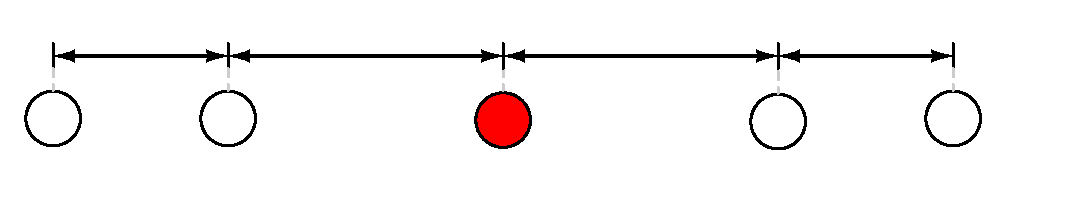
\includegraphics[scale=1]{config6}\\
   % translate x=548 y=272 scale 0.38
   \putbox{3.2in}{0.08in}{1.20}{$\lambda$}%
   \putbox{4.99in}{0.06in}{1.20}{$\lambda/2$}%
   \putbox{2.04in}{0.97in}{1.20}{$\lambda/2$}%
   \putbox{1.22in}{0.08in}{1.20}{$\lambda/2$}%
   \putbox{6.1in}{0.08in}{1.20}{$\lambda/4$}%
   \putbox{0.66in}{0.97in}{1.20}{$\lambda/4$}%
   \putbox{5.5in}{0.95in}{1.20}{$\lambda/4$}%
   \putbox{0.06in}{0.08in}{1.20}{$\lambda/4$}%
   \putbox{4in}{0.95in}{1.20}{$\lambda/2$}%
   } % close 'parbox'
   } % close 'scalebox'
   \vspace{-\baselineskip} % this is not necessary, but looks better
}
	\caption{Configuración 6 asignada en dirección $z$.}
	\label{fig.config_z}
\end{figure}	


La figura \ref{fig.config_z} muestra la configuración de radiadores asignada vista desde arriba (plano xy), la misma consiste en un conjunto de conductores formada por alambres, de los cuales sólo uno de ellos (de color rojo) es activo, es decir se encuentra conectado a una funete de tensión de \SI{1}{\volt}. Los cuatro conductores restantes son pasivos, pudiendo funcionar como directores o reflectores. El radio de todos los conductores es de \SI{5}{\milli\meter}.
La longitud y distancias entre conductores están expresadas en términos de longitud de onda para la frecuencia más pequeña. El rango de fercuencias a analizar es $\SI{80}{\mega\hertz} < f < \SI{480}{\mega\hertz}$, por lo que se puede deducir el valor de una longitud de onda según la expresión \eqref{ec.long_onda}, sinedo $\rm{c}=\SI{3e8}{\meter\per\second}$ la velocidad de propagación de la onda en espacio libre.

\begin{equation}
	\centering
	\lambda = \frac{\rm{c}}{\rm{f_{min}}} = \frac{ \SI{3e8}{\meter\per\second} } { \SI{80}{\mega\hertz} } = \SI{3.75}{\meter}
	\label{ec.long_onda}
\end{equation} 

\begin{figure}[H]
	\begin{subfigure}{0.5\textwidth}
		\scalebox{0.7}{% XCircuit output "config6xy.tex" for LaTeX input from config6xy.ps
\def\putbox#1#2#3#4{\makebox[0in][l]{\makebox[#1][l]{}\raisebox{\baselineskip}[0in][0in]{\raisebox{#2}[0in][0in]{\scalebox{#3}{#4}}}}}
\def\rightbox#1{\makebox[0in][r]{#1}}
\def\centbox#1{\makebox[0in]{#1}}
\def\topbox#1{\raisebox{-0.60\baselineskip}[0in][0in]{#1}}
\def\midbox#1{\raisebox{-0.20\baselineskip}[0in][0in]{#1}}
   \scalebox{1}{
   \normalsize
   \parbox{4.1875in}{
   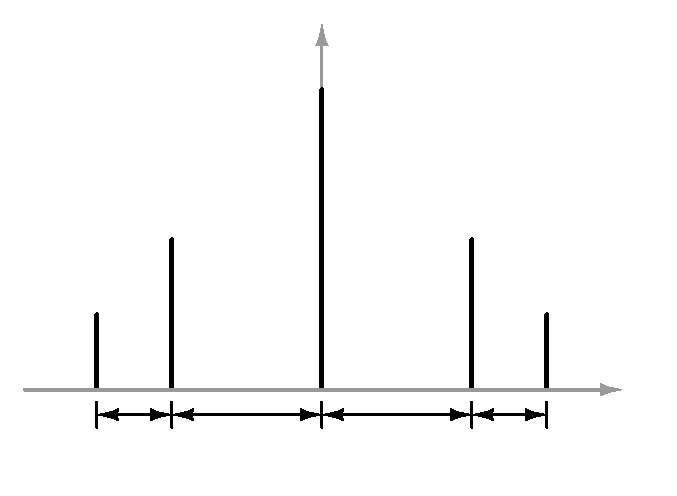
\includegraphics[scale=1]{config6xy}\\
   % translate x=540 y=424 scale 0.38
   \putbox{1.85in}{0.7in}{1.20}{\rotatebox{-270}{\tiny{$\lambda = \SI{3.75}{\meter}$}}}%
   \putbox{0.85in}{0.7in}{1.20}{\rotatebox{-270}{\tiny{$\lambda /2 = \SI{1.875}{\meter}$}}}%
   \putbox{0.35in}{0.7in}{1.20}{\rotatebox{-270}{\tiny{$\lambda /4 = \SI{0.9375}{\meter}$}}}%
   \putbox{2.85in}{0.7in}{1.20}{\rotatebox{-270}{\tiny{$\lambda /2 = \SI{1.875}{\meter}$}}}%
   \putbox{3.4in}{0.7in}{1.20}{\rotatebox{-270}{\tiny{$\lambda /4 = \SI{0.9375}{\meter}$}}}%
   \putbox{2.14in}{2.89in}{1.20}{$z$}%
   \putbox{4.14in}{0.56in}{1.20}{$x$}%
   \putbox{1.2in}{0.26in}{1.20}{{\tiny{$\lambda /2 = \SI{1.875}{\meter}$}}}%
   \putbox{2.2in}{0.26in}{1.20}{{\tiny{$\lambda /2 = \SI{1.875}{\meter}$}}}%
   \putbox{0.58in}{0.26in}{1.20}{\tiny{$\lambda /4=$}}%
   \putbox{3.18in}{0.26in}{1.20}{\tiny{$\lambda /4=$}}%
   \putbox{0.5in}{0.15in}{1.20}{\tiny{$\SI{0.9375}{\meter}$}}%
   \putbox{3.1in}{0.15in}{1.20}{\tiny{$\SI{0.9375}{\meter}$}}%
   } % close 'parbox'
   } % close 'scalebox'
   \vspace{-\baselineskip} % this is not necessary, but looks better
}
		\caption{Configuración 6 asignada (plano $xz$).}
		\label{fig.config_xz}
	\end{subfigure}
	\quad
	\begin{subfigure}{0.5\textwidth}
		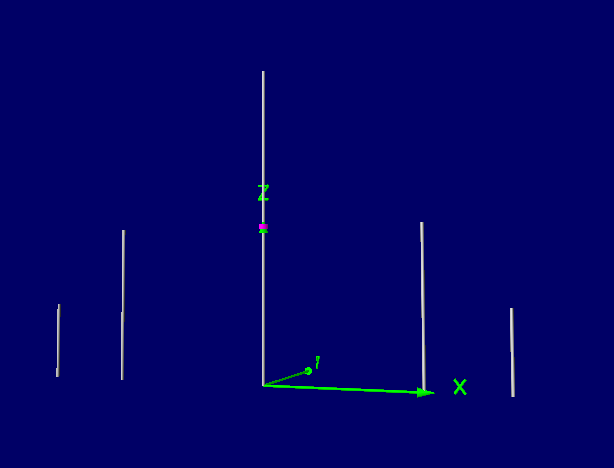
\includegraphics[scale=0.4]{imagenes/2_geometria.png}
		\caption{Geometría ingresada en el programa \textit{4nec2}.}
		\label{fig.geometria}
	\end{subfigure}
\end{figure}
 
Por lo tanto la configuración en el plano xz con las medidas correspondientes se muestra en \ref{fig.config_xz}. La figura \ref{fig.geometria} muestra la geometría ingresada en el programa \textit{4nec2}, en espacio libre. El punto rosa en el conductor central indica la fuente (que es de \SI{1}{\volt}) y se ubicó en su posición central.   








		\subsection{Diagramas de radiación}
			\begin{figure}[H]
	\begin{subfigure}{0.5\textwidth}
		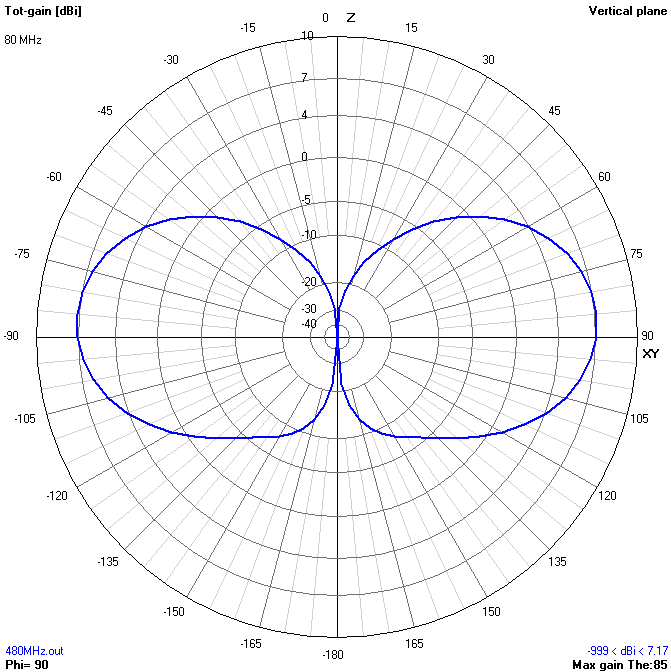
\includegraphics[scale=0.43]{imagenes/2D_80MHz.png}
	\end{subfigure}	
	\quad
	\begin{subfigure}{0.5\textwidth}
		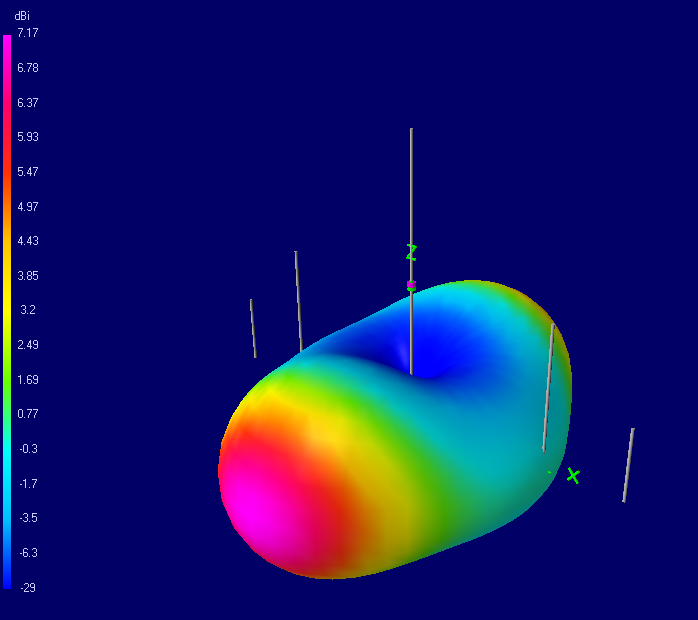
\includegraphics[scale=0.43]{imagenes/3D_80MHz.png}
	\end{subfigure}
	\caption{$f=\SI{80}{\mega\hertz}$}
	\label{fig.radiacion_80M}
\end{figure}


\begin{figure}[H]
	\begin{subfigure}{0.5\textwidth}
		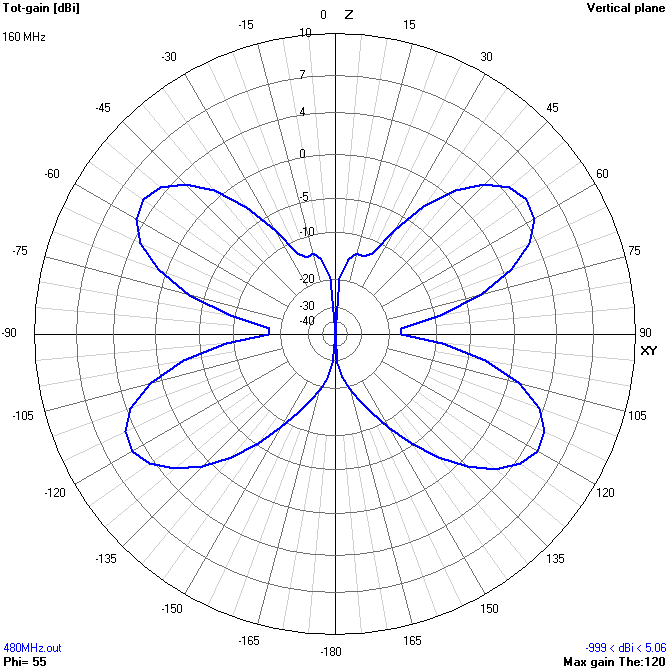
\includegraphics[scale=0.43]{imagenes/2D_160MHz.png}
	\end{subfigure}	
	\quad
	\begin{subfigure}{0.5\textwidth}
		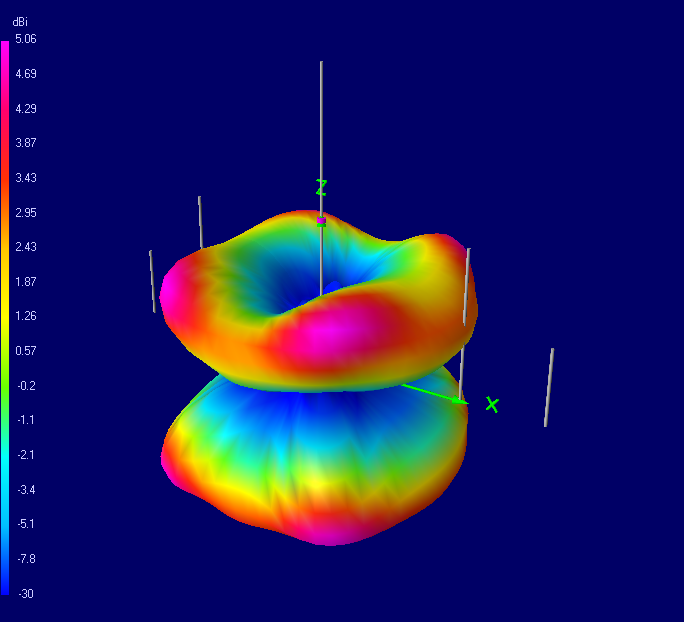
\includegraphics[scale=0.43]{imagenes/3D_160MHz.png}
	\end{subfigure}
	\caption{$f=\SI{160}{\mega\hertz}$}
	\label{fig.radiacion_160M}
\end{figure}


\begin{figure}[H]
	\begin{subfigure}{0.5\textwidth}
		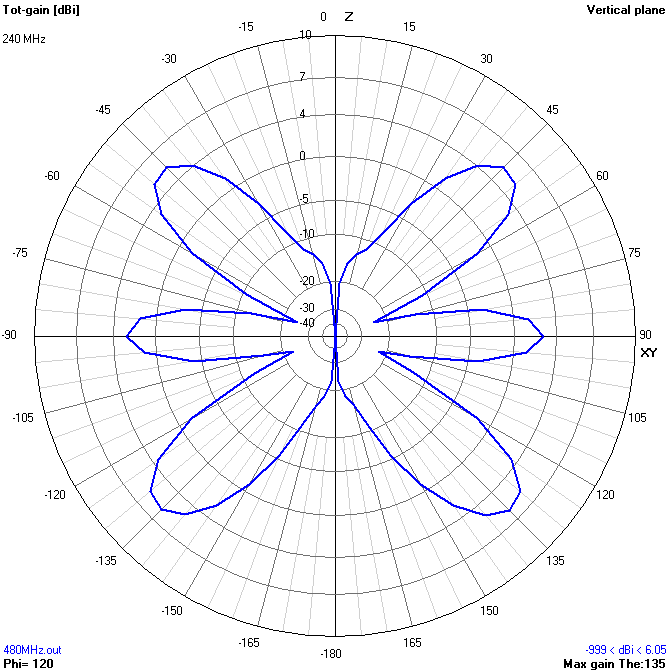
\includegraphics[scale=0.43]{imagenes/2D_240MHz.png}
	\end{subfigure}	
	\quad
	\begin{subfigure}{0.5\textwidth}
		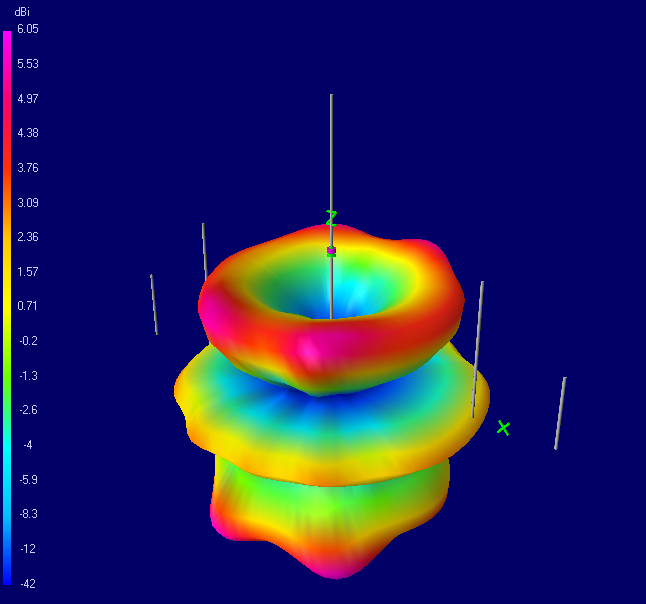
\includegraphics[scale=0.43]{imagenes/3D_240MHz.png}
	\end{subfigure}
	\caption{$f=\SI{240}{\mega\hertz}$}
	\label{fig.radiacion_240M}
\end{figure}


\begin{figure}[H]
	\begin{subfigure}{0.5\textwidth}
		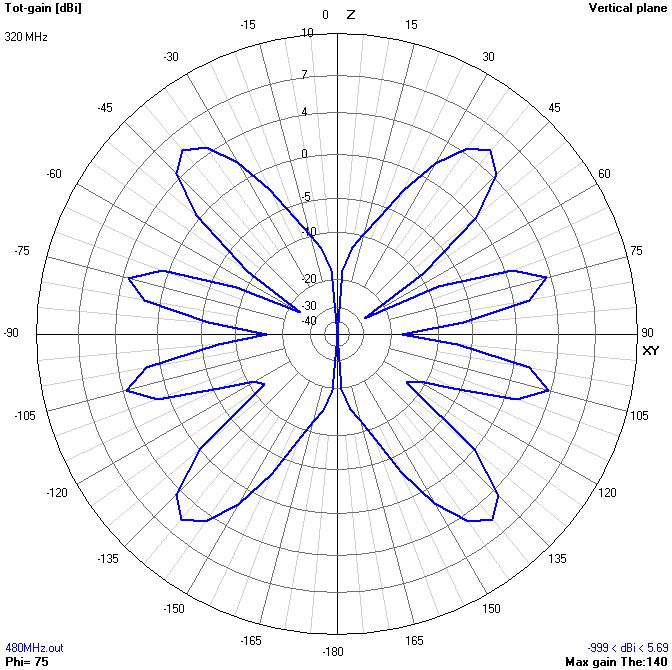
\includegraphics[scale=0.43]{imagenes/2D_320MHz.png}
	\end{subfigure}	
	\quad
	\begin{subfigure}{0.5\textwidth}
		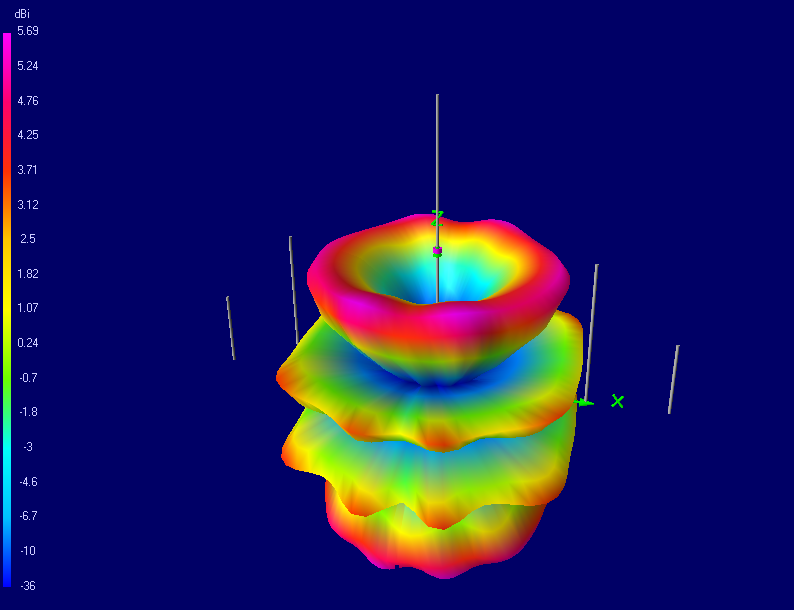
\includegraphics[scale=0.43]{imagenes/3D_320MHz.png}
	\end{subfigure}
	\caption{$f=\SI{320}{\mega\hertz}$.}
	\label{fig.radiacion_320M}
\end{figure}


\begin{figure}[H]
	\begin{subfigure}{0.5\textwidth}
		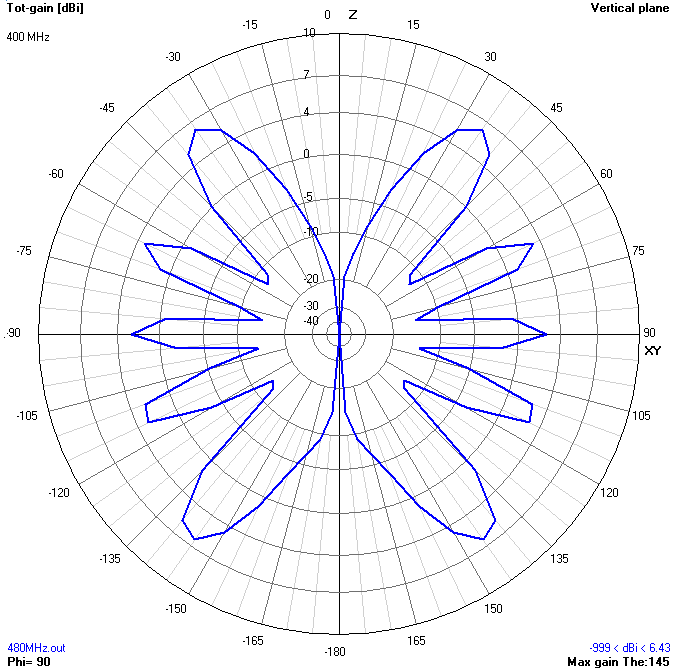
\includegraphics[scale=0.43]{imagenes/2D_400MHz.png}
	\end{subfigure}	
	\quad
	\begin{subfigure}{0.5\textwidth}
		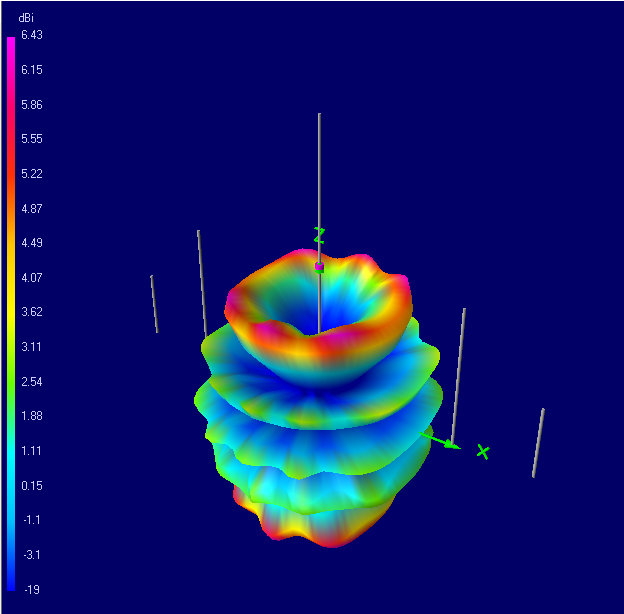
\includegraphics[scale=0.43]{imagenes/3D_400MHz.png}
	\end{subfigure}
	\caption{$f=\SI{400}{\mega\hertz}$.}
	\label{fig.radiacion_320M}
\end{figure}



\begin{figure}[H]
	\begin{subfigure}{0.5\textwidth}
		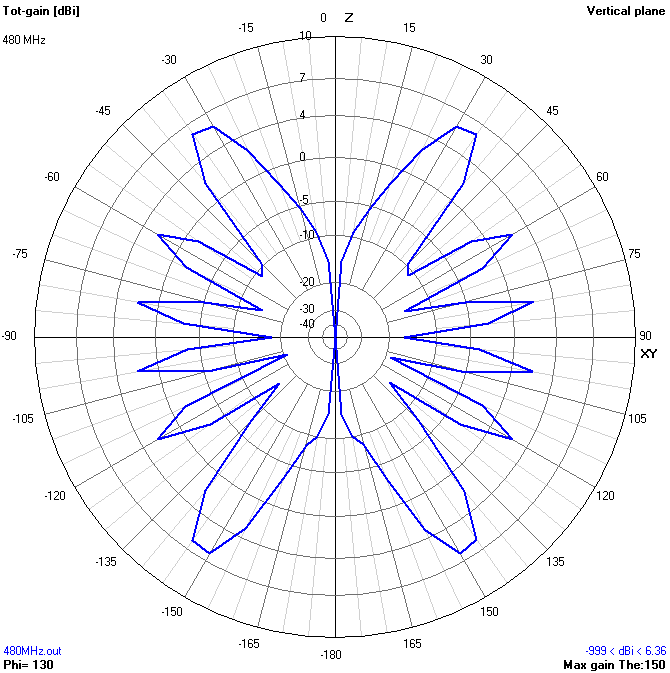
\includegraphics[scale=0.43]{imagenes/2D_480MHz.png}
	\end{subfigure}	
	\quad
	\begin{subfigure}{0.5\textwidth}
		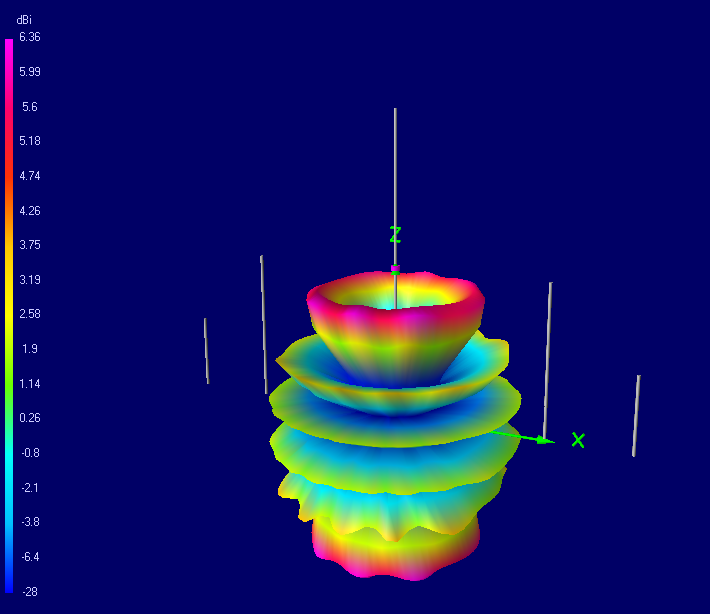
\includegraphics[scale=0.43]{imagenes/3D_480MHz.png}
	\end{subfigure}
	\caption{$f=\SI{480}{\mega\hertz}$.}
	\label{fig.radiacion_480M}
\end{figure}	
		\subsection{Gráfico de corriente}
			%\begin{figure}[H]
%	\begin{subfigure}{0.5\textwidth}
%		\input{imagenes/i_real_80.eps}
%		%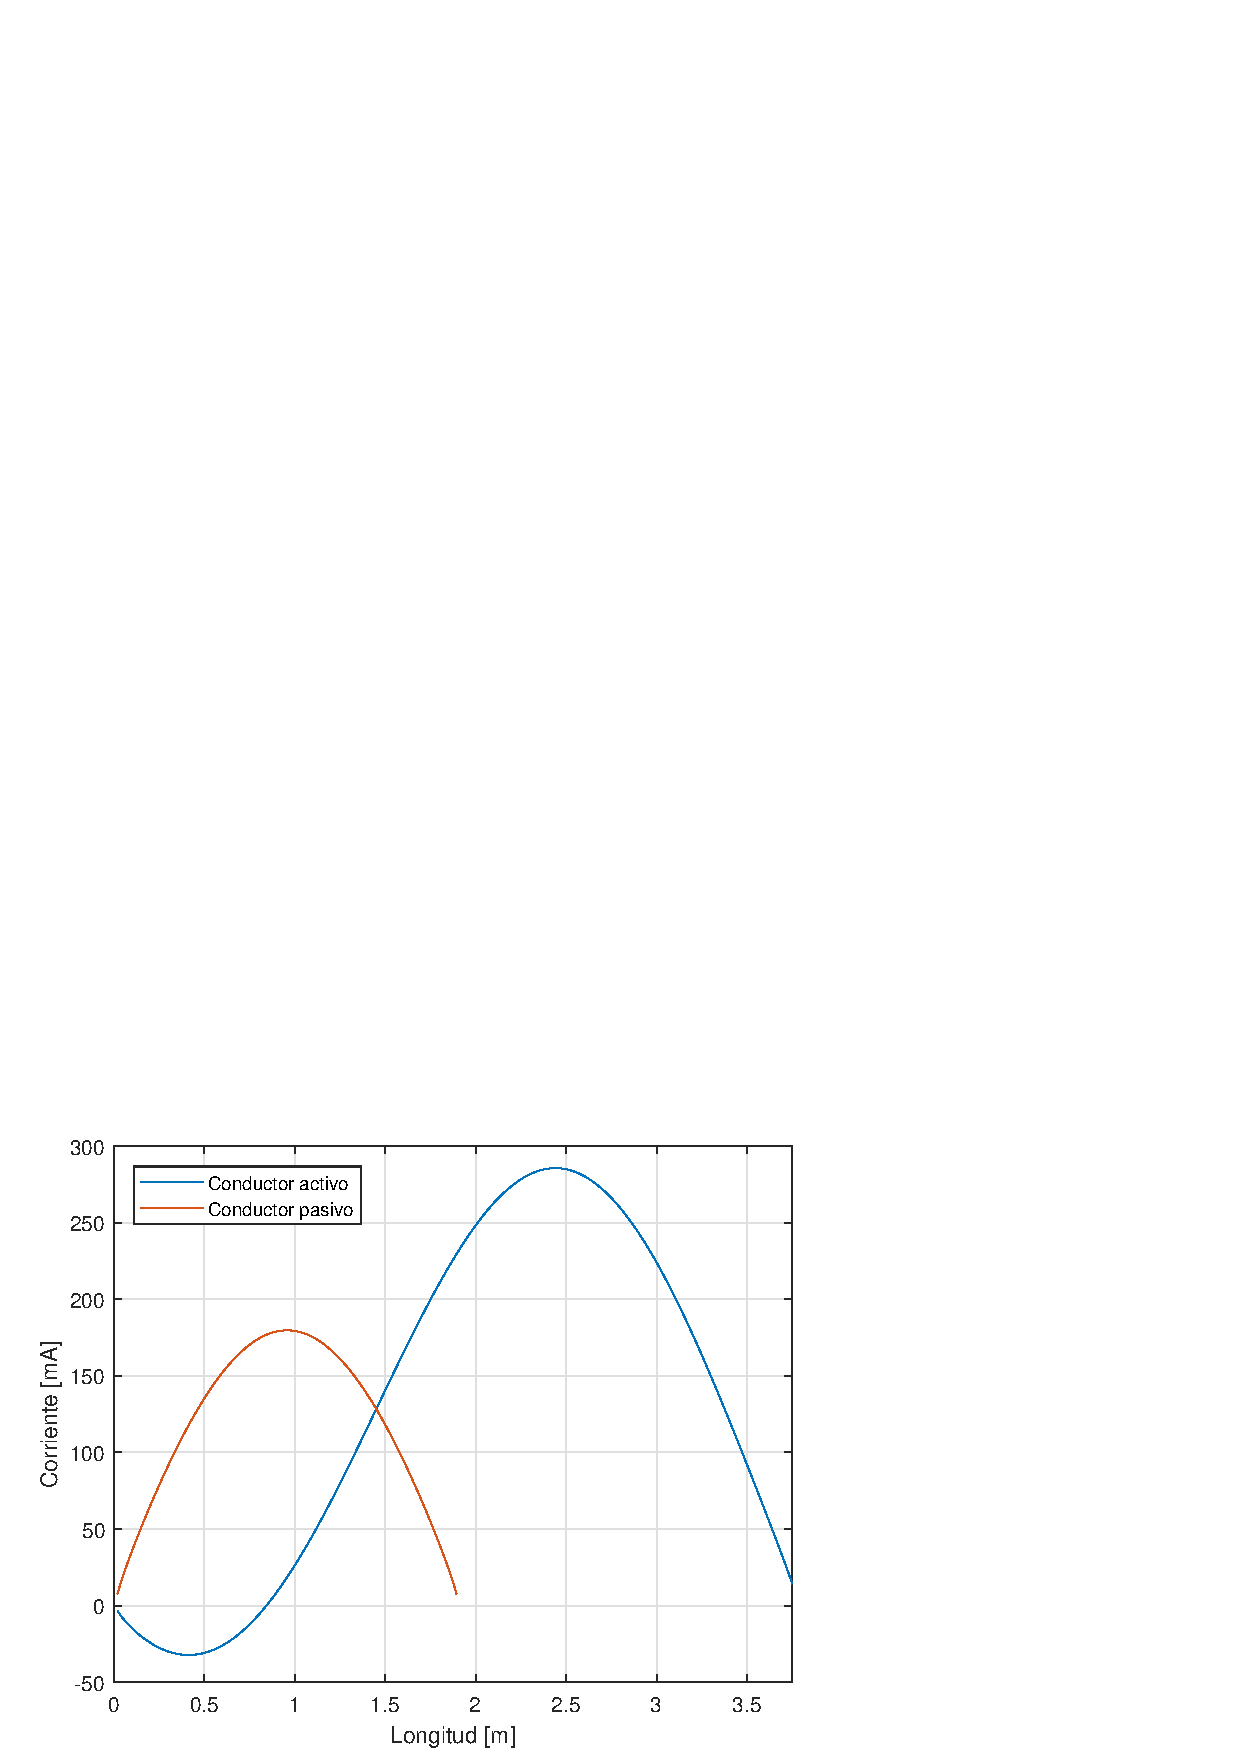
\includegraphics[scale=0.43]{imagenes/i_real_80.png}
%		%\caption{Parte real de la corriente.}
%	\end{subfigure}	
%	\quad
%	\begin{subfigure}{0.5\textwidth}
%		\input{imagenes/i_imag_80.eps}
%		%\includegraphics[scale=0.43]{imagenes/i_imag.png}
%		%\caption{Parte imaginaria de la corriente.}
%	\end{subfigure}
%	\caption{$f=\SI{80}{\mega\hertz}$}
%	\label{fig.corriente_80M_real_imag}
%\end{figure}

\begin{figure}[H]
	\begin{subfigure}{0.5\textwidth}
		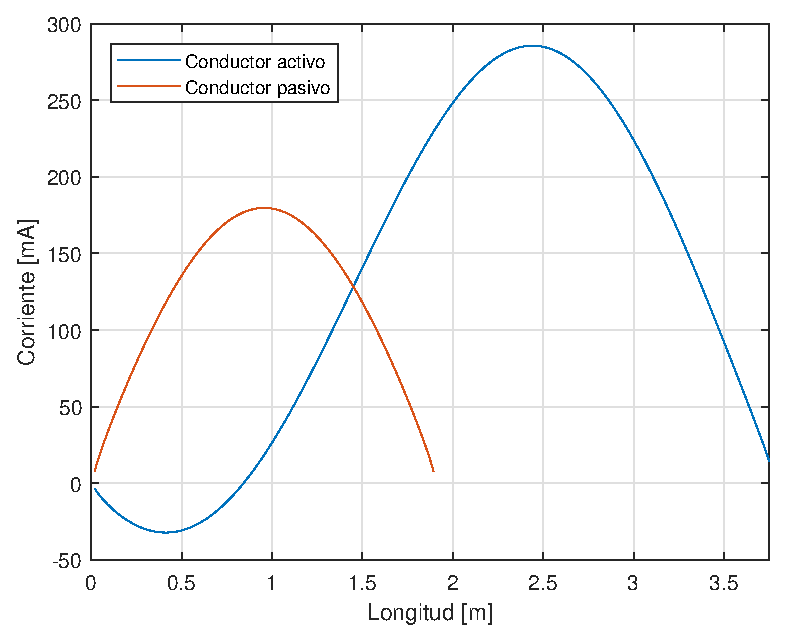
\includegraphics[scale=0.6]{imagenes/i_real_80.eps}
		\caption{Parte real.}
	\end{subfigure}
	\quad
	\begin{subfigure}{0.5\textwidth}
		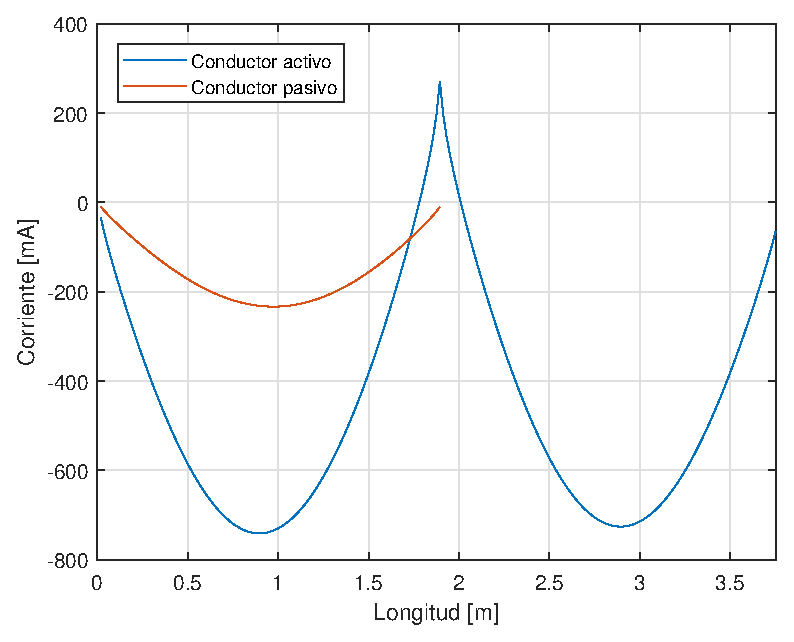
\includegraphics[scale=0.6]{imagenes/i_imag_80.eps}
		\caption{Parte imaginaria.}
	\end{subfigure}
	\quad
	\begin{subfigure}{0.5\textwidth}
		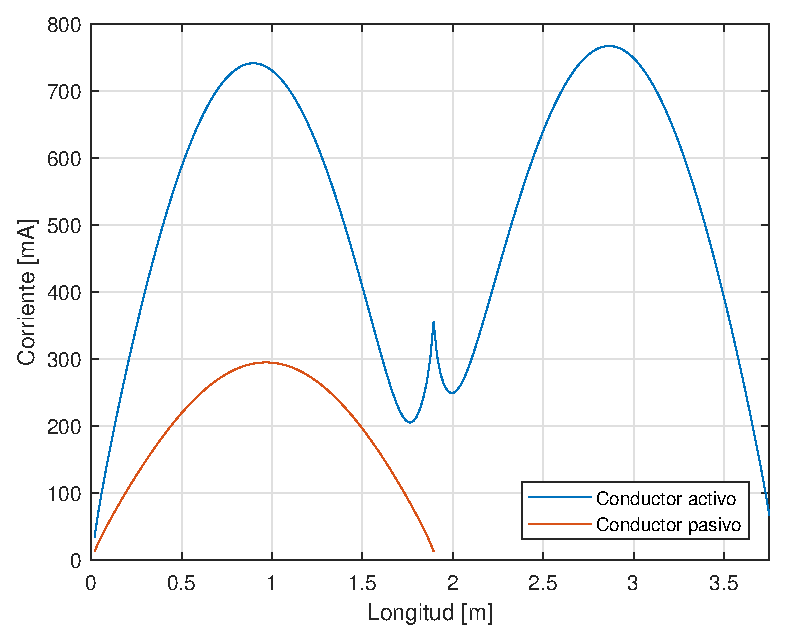
\includegraphics[scale=0.6]{imagenes/i_mag_80.eps}
		\caption{Magnitud.}
	\end{subfigure}
	\quad
	\begin{subfigure}{0.5\textwidth}
		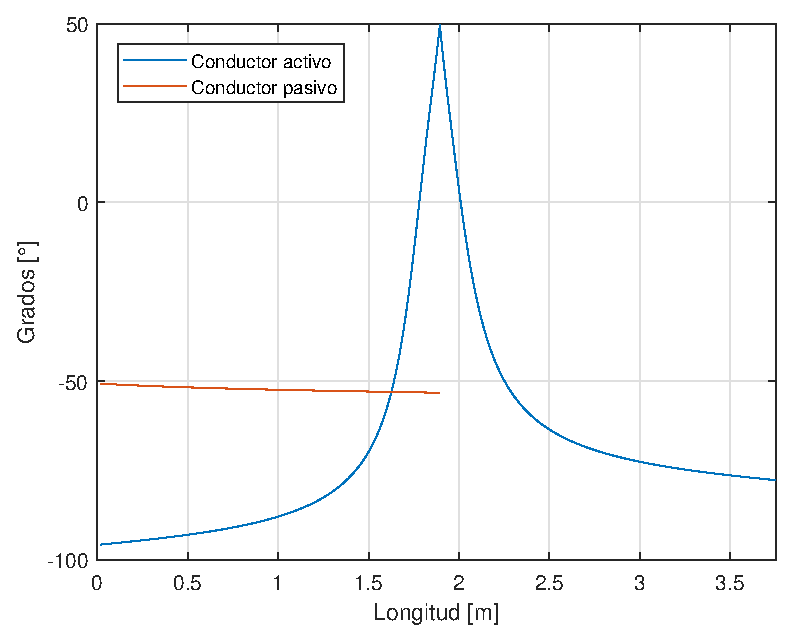
\includegraphics[scale=0.6]{imagenes/i_fase_80.eps}
		\caption{Fase.}
	\end{subfigure}
	\caption{Corriente para la frecuencia mínima $f = \SI{80}{\mega\hertz}$}
\end{figure}


\begin{figure}[H]
	\begin{subfigure}{0.5\textwidth}
		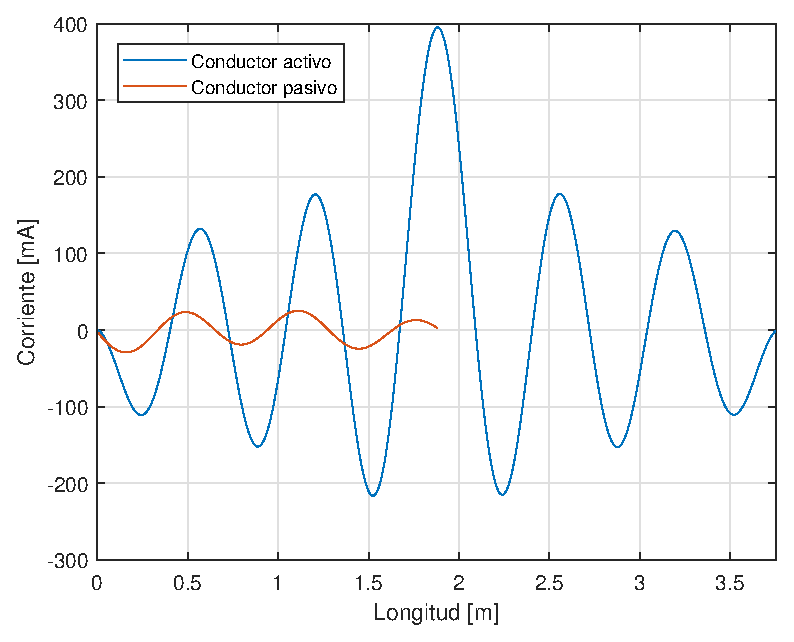
\includegraphics[scale=0.6]{imagenes/i_real_480.eps}
		\caption{Parte real.}
	\end{subfigure}
	\quad
	\begin{subfigure}{0.5\textwidth}
		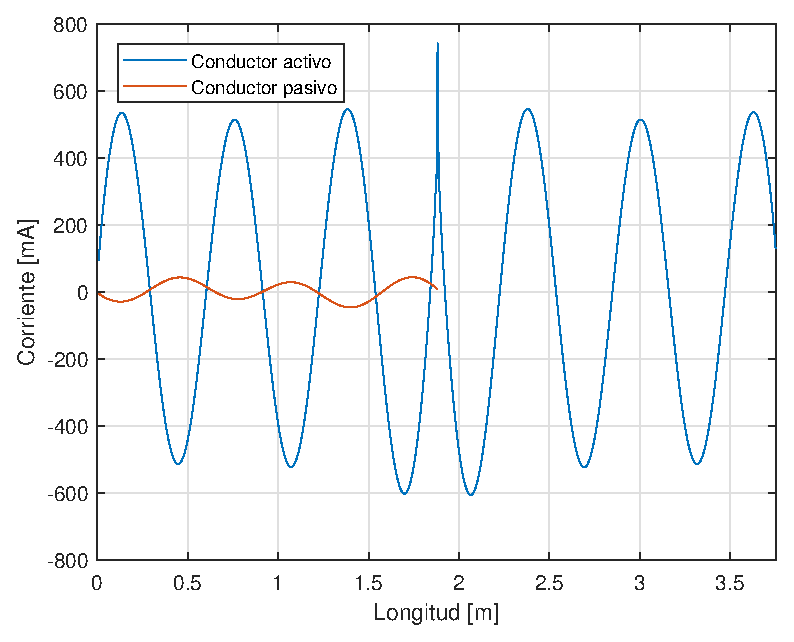
\includegraphics[scale=0.6]{imagenes/i_imag_480.eps}
		\caption{Parte imaginaria.}
	\end{subfigure}
	\quad
	\begin{subfigure}{0.5\textwidth}
		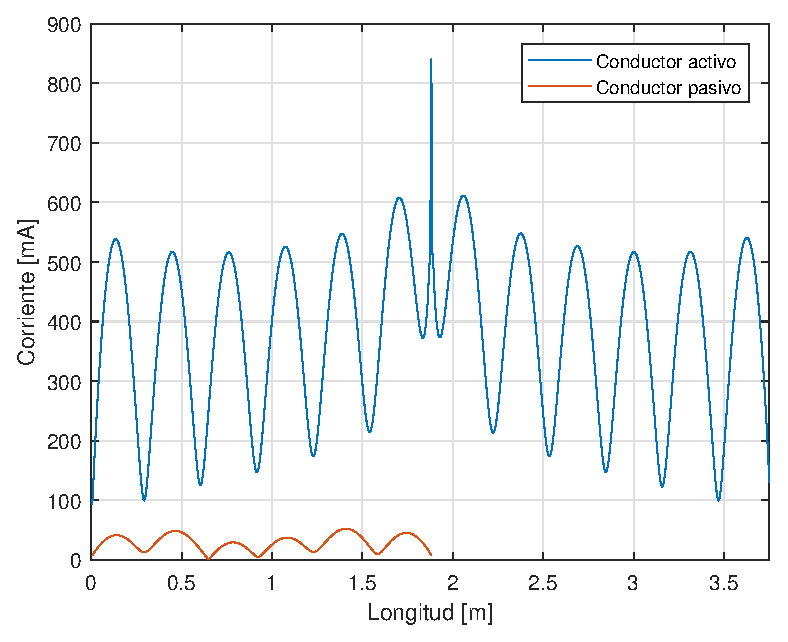
\includegraphics[scale=0.6]{imagenes/i_mag_480.eps}
		\caption{Magnitud.}
	\end{subfigure}
	\quad
	\begin{subfigure}{0.5\textwidth}
		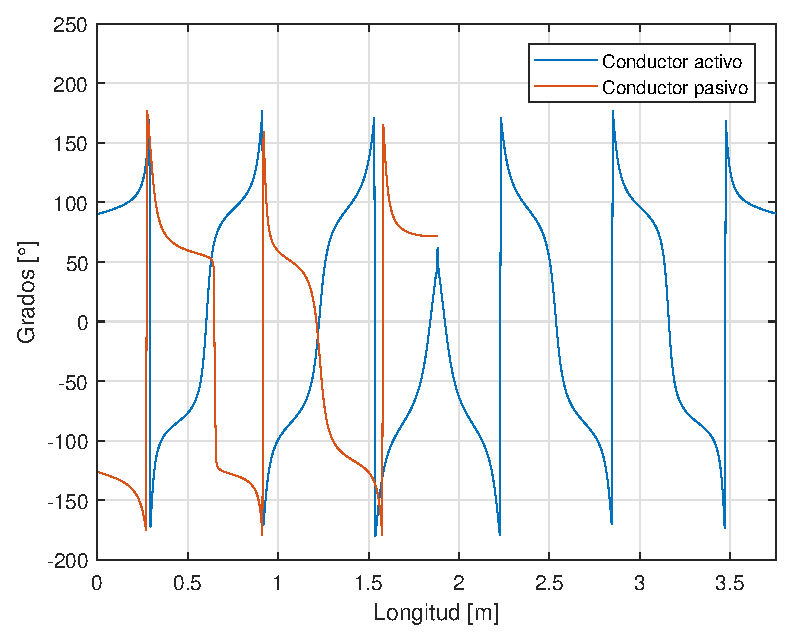
\includegraphics[scale=0.6]{imagenes/i_fase_480.eps}
		\caption{Fase.}
	\end{subfigure}
	\caption{Corriente para la frecuencia máxima $f = \SI{480}{\mega\hertz}$}
\end{figure}



		\subsection{Resistencia de radiación}
			\begin{figure}[H]
	\centering
	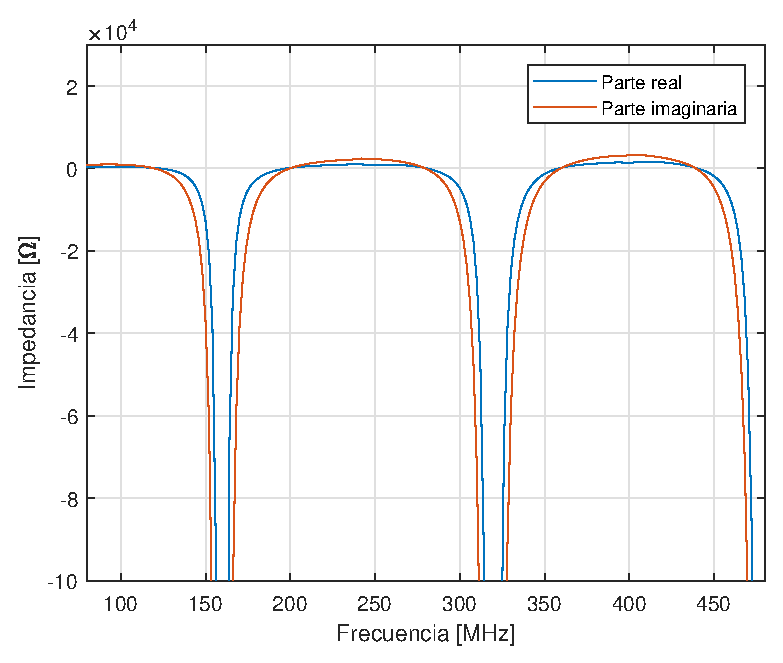
\includegraphics{imagenes/z.eps}
	\caption{Resistencia de radiación.}
	\label{fig.z_radiacion}
\end{figure}
		\subsection{Diseño de adaptador de impedancia}
			La adaptación permite obtener una máxima eficiencia en la transmisión de energía, eliminando reflexiones de onda. Dentro de las posibles formas de adaptación, se optó por la utilización del adaptador de cuarto de onda y stub. La línea opera en un entorno de la mínima frecuencia, $\SI{72}{\mega\hertz} < f < \SI{88}{\mega\hertz}$, por lo que se considera el valor de carga de la expresión \eqref{ec.z_80}.

A su vez se considera un criterio de $|\rho_l|<0,2$, ó de forma equivalente $\rm{ROE} \leq 1,5$

\subsection{Adaptador de cuarto de onda}
El proceso consiste en intercalar el adaptador a una distancia $z_s$ de la carga $Z_L$, de forma tal que la impedancia de entrada $Z_{in}$ del conjunto línea y carga sea real. Para hallar el valor de $z_s$ se utiliza la carta de Smith mediante software. El adaptador queda definido mediante los parámetros $z_a$ (impedancia del adaptador) y $L_a$ (longitud del adaptador). La impedancia característica de la línea es dato, $Z_o = \SI{50}{\ohm}$. Ubicandose en $Z_L$, se desplaza hacia el generador sobre la circuinferencia $|\rho_L|$ hasta obtener impedancia real (eje real). Así se obtiene longitud de arco recorrido da la posición $z_s$ del adaptador. A partir de dicho valor y $Z_{in}$ se obtienen los parámetros de la línea \eqref{ec.z_a_4} y \eqref{ec.L_a_4}.

\begin{equation}
	\centering
	Z_a = \sqrt{Z_o \cdot Z_{in}} = \sqrt{ \SI{50}{\ohm} \cdot \SI{1.38}{\ohm} } = \SI{8.3}{\ohm}
	\label{ec.z_a_4}
\end{equation}	

\begin{equation}
	\centering
	L_a = \frac{\lambda_a}{4} = \frac{ \SI{3.75}{\meter} }{4} = \SI{0.937}{\meter}
	\label{ec.L_a_4}
\end{equation}

%%%% FIGURA PARA CUARTO DE ONDA ESPACIO LIBRE
\begin{figure}[H]
	\centering
	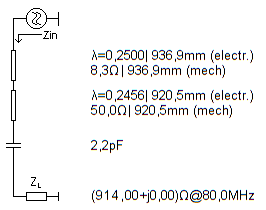
\includegraphics[scale=0.83]{imagenes/smith_4_espacio_libre_esq.png}
	\label{fig.smith_4_esq}
\end{figure}
\begin{figure}[H]
	\centering
	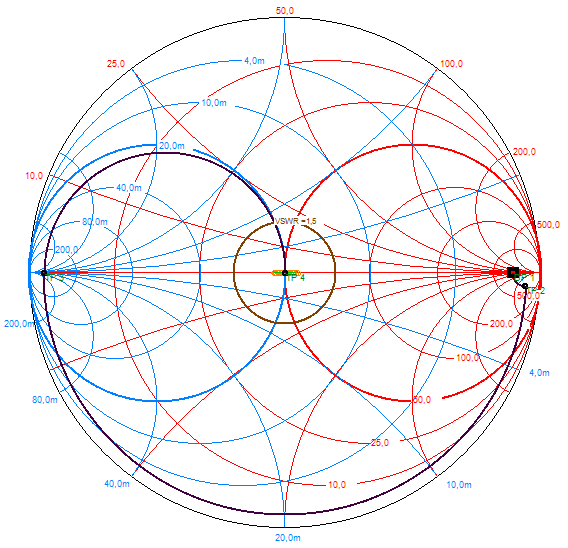
\includegraphics[scale=0.63]{imagenes/smith_4_espacio_libre.png}
	\label{fig.smith_4}
\end{figure}



\subsection{Stub}

La adaptación mediante \texttt{stub} consiste en anexar un trozo de la misma línea conectada en paralelo. Normalmente, para evitar interferencias se suele cortocircuitar el extremo de la carga. Se parte del punto de impedancia obtenido en \emph{4nec2} hasta llegar a la circunferencia de impedancia real unitaria moviéndose hacia el generador. Allí se coloca el stub cuyo largo será el necesario hasta llegar al centro de la carta recorriendo la circunferencia de impedancia real unitaria en sentido antihorario. Utilizando el programa se obtiene:

\begin{equation*}
	\centering
	L_s = \num{0.0269}\cdot \lambda = \SI{100.8}{\milli\m}
\end{equation*}

\begin{equation*}
	\centering
	d_s = \num{0.2195}\cdot \lambda = \SI{822.5}{\milli\m}
\end{equation*}


%%%% FIGURA PARA STUB ESPACIO LIBRE
\begin{figure}[H]
	\centering
	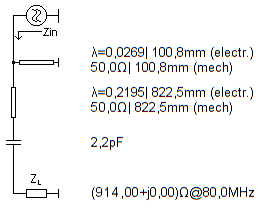
\includegraphics[scale=0.83]{imagenes/smith_stub_espacio_libre_esq.png}
	\label{fig.smith_stub_esq}
\end{figure}

\begin{figure}[H]
	\centering
	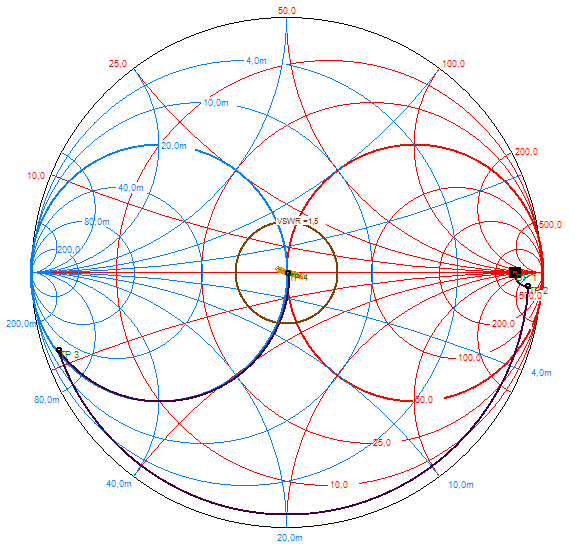
\includegraphics[scale=0.63]{imagenes/smith_stub_espacio_libre.png}
	\label{fig.smith_stub}
\end{figure}




		\subsection{Plano de tierra perfecto}
			%%%%%%%%%% 2. Geometría %%%%%%%%%%%%

\begin{figure}[H]
	\centering
	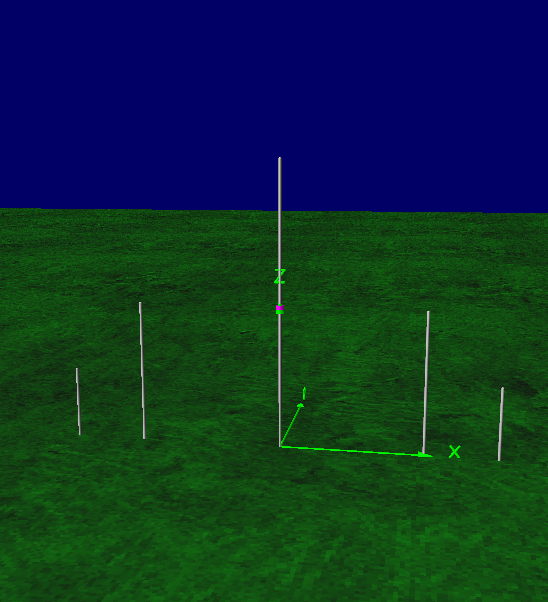
\includegraphics[scale=0.4]{imagenes/2_geometria_tierra.png}
	\caption{Geometría ingresada con plano a tierra perfecto.}
	\label{fig.geometria_tierra}
\end{figure}

%%%%%%%%%% 3. Diagramas de radiación %%%%%%%%%%

\begin{figure}[H]
	\begin{subfigure}{0.5\textwidth}
		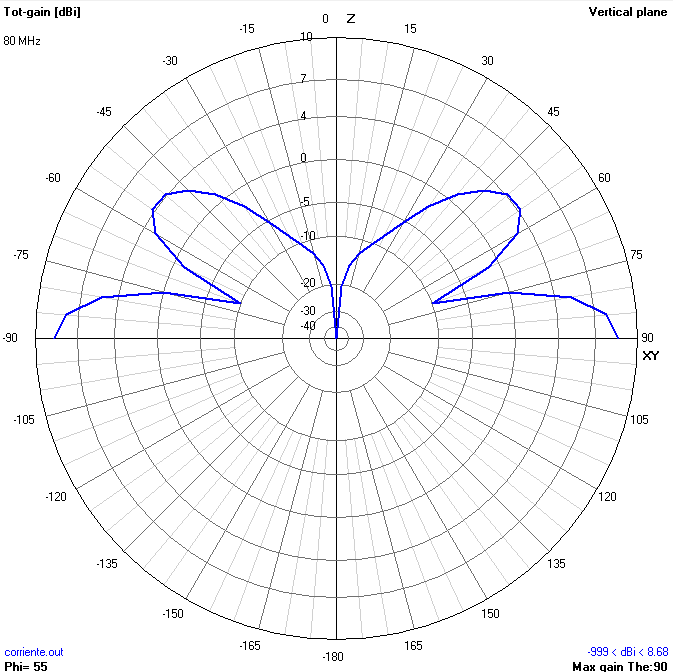
\includegraphics[scale=0.43]{imagenes/2D_80MHz_tierra.png}
	\end{subfigure}	
	\quad
	\begin{subfigure}{0.5\textwidth}
		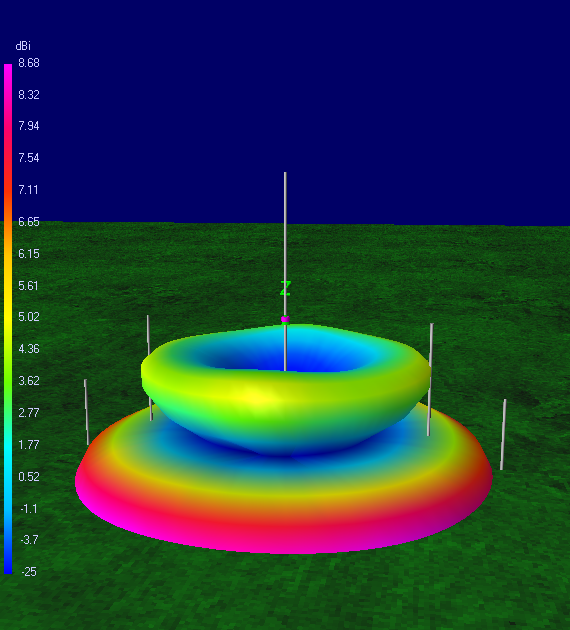
\includegraphics[scale=0.43]{imagenes/3D_80MHz_tierra.png}
	\end{subfigure}
	\caption{$f=\SI{80}{\mega\hertz}$}
	\label{fig.radiacion_80M_tierra}
\end{figure}


\begin{figure}[H]
	\begin{subfigure}{0.5\textwidth}
		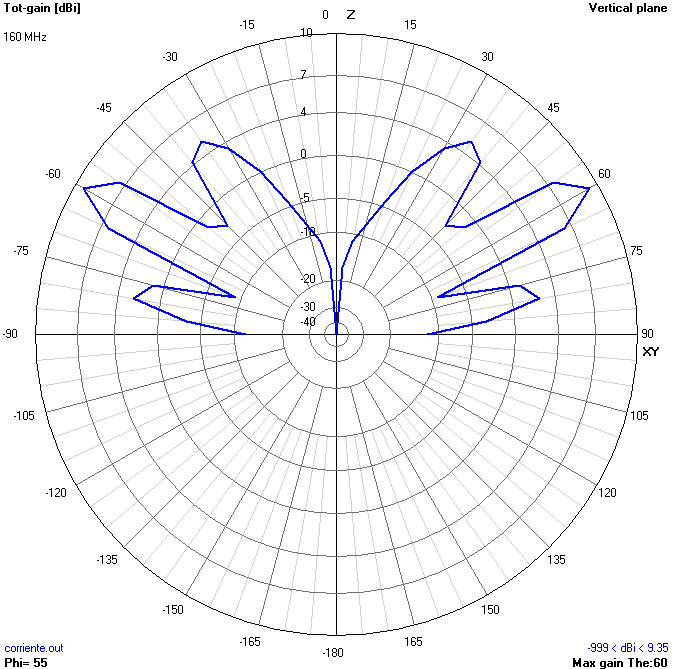
\includegraphics[scale=0.43]{imagenes/2D_160MHz_tierra.png}
	\end{subfigure}	
	\quad
	\begin{subfigure}{0.5\textwidth}
		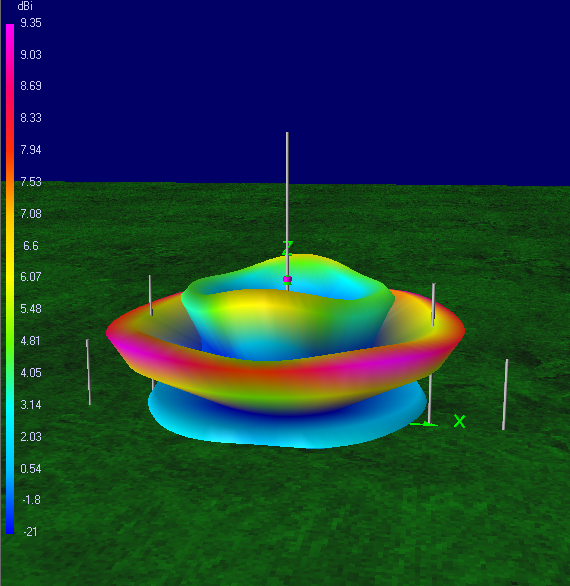
\includegraphics[scale=0.43]{imagenes/3D_160MHz_tierra.png}
	\end{subfigure}
	\caption{$f=\SI{160}{\mega\hertz}$}
	\label{fig.radiacion_160M_tierra}
\end{figure}


\begin{figure}[H]
	\begin{subfigure}{0.5\textwidth}
		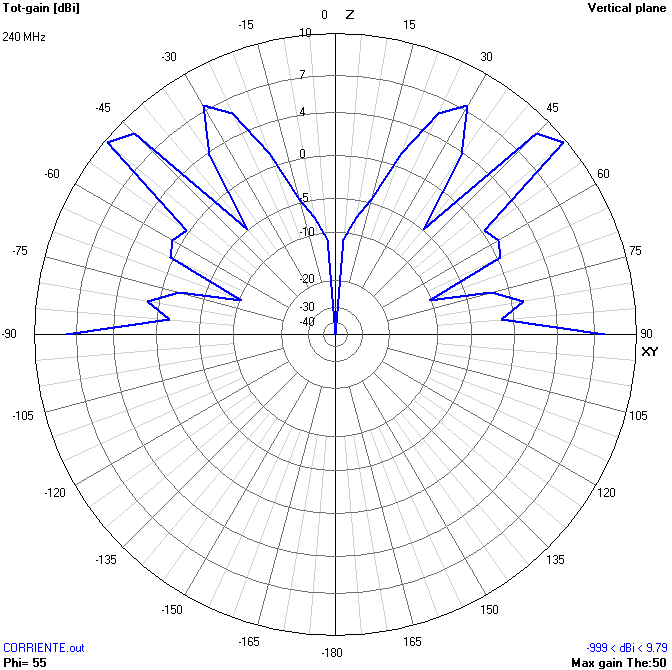
\includegraphics[scale=0.43]{imagenes/2D_240MHz_tierra.png}
	\end{subfigure}	
	\quad
	\begin{subfigure}{0.5\textwidth}
		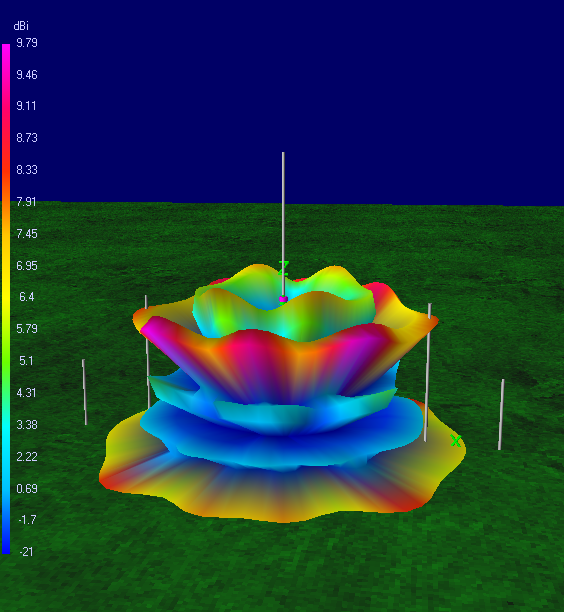
\includegraphics[scale=0.43]{imagenes/3D_240MHz_tierra.png}
	\end{subfigure}
	\caption{$f=\SI{240}{\mega\hertz}$}
	\label{fig.radiacion_240M_tierra}
\end{figure}


\begin{figure}[H]
	\begin{subfigure}{0.5\textwidth}
		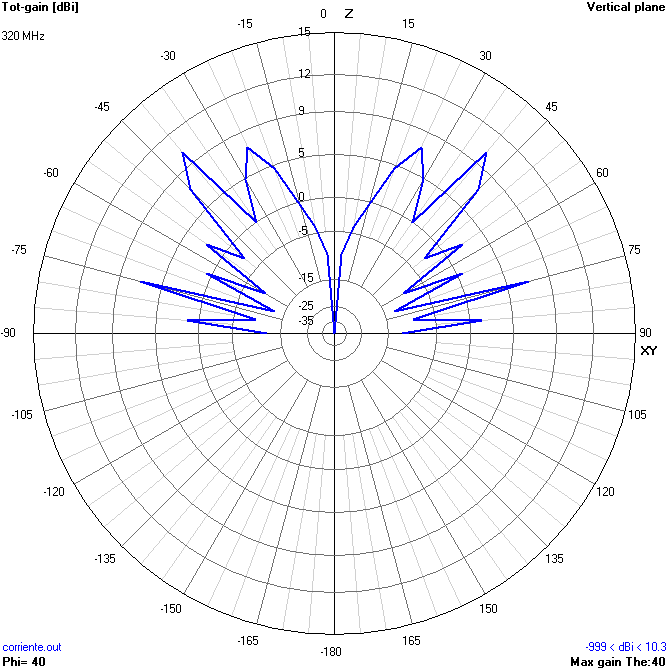
\includegraphics[scale=0.43]{imagenes/2D_320MHz_tierra.png}
	\end{subfigure}	
	\quad
	\begin{subfigure}{0.5\textwidth}
		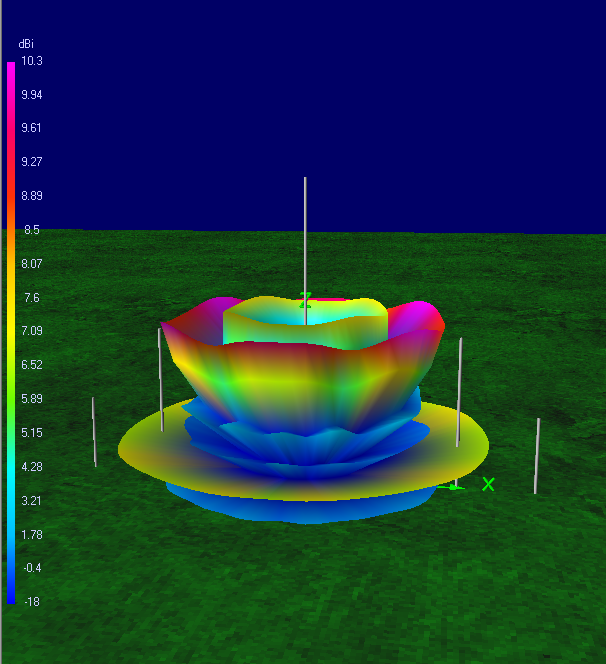
\includegraphics[scale=0.43]{imagenes/3D_320MHz_tierra.png}
	\end{subfigure}
	\caption{$f=\SI{320}{\mega\hertz}$.}
	\label{fig.radiacion_320M_tierra}
\end{figure}


\begin{figure}[H]
	\begin{subfigure}{0.5\textwidth}
		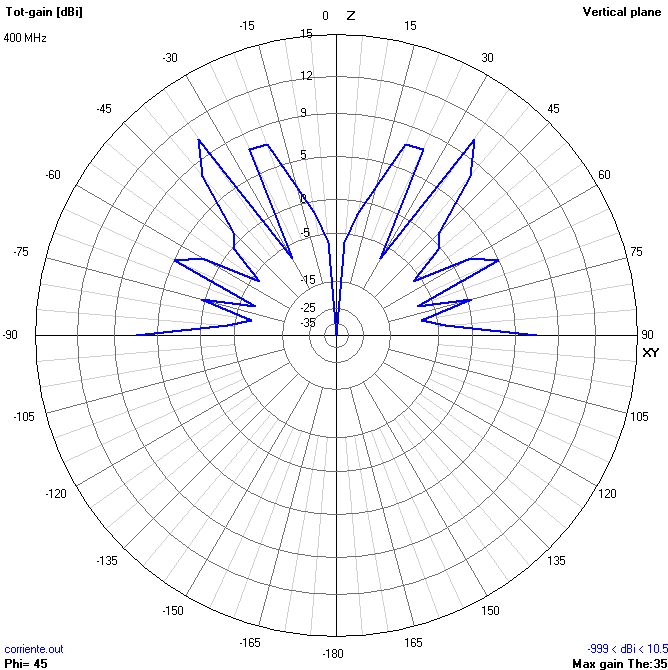
\includegraphics[scale=0.43]{imagenes/2D_400MHz_tierra.png}
	\end{subfigure}	
	\quad
	\begin{subfigure}{0.5\textwidth}
		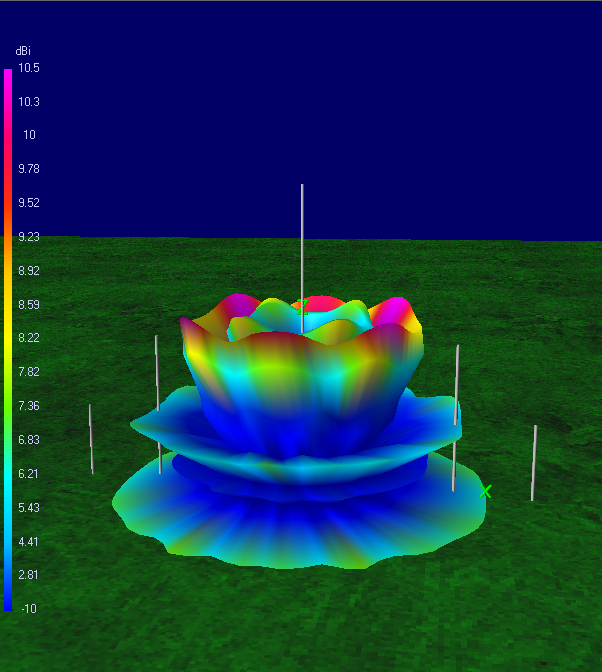
\includegraphics[scale=0.43]{imagenes/3D_400MHz_tierra.png}
	\end{subfigure}
	\caption{$f=\SI{400}{\mega\hertz}$.}
	\label{fig.radiacion_400M_tierra}
\end{figure}



\begin{figure}[H]
	\begin{subfigure}{0.5\textwidth}
		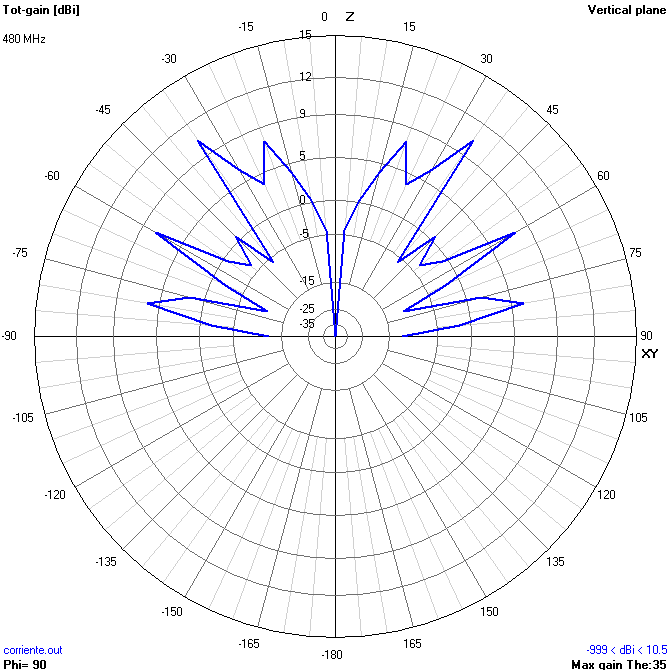
\includegraphics[scale=0.43]{imagenes/2D_480MHz_tierra.png}
	\end{subfigure}	
	\quad
	\begin{subfigure}{0.5\textwidth}
		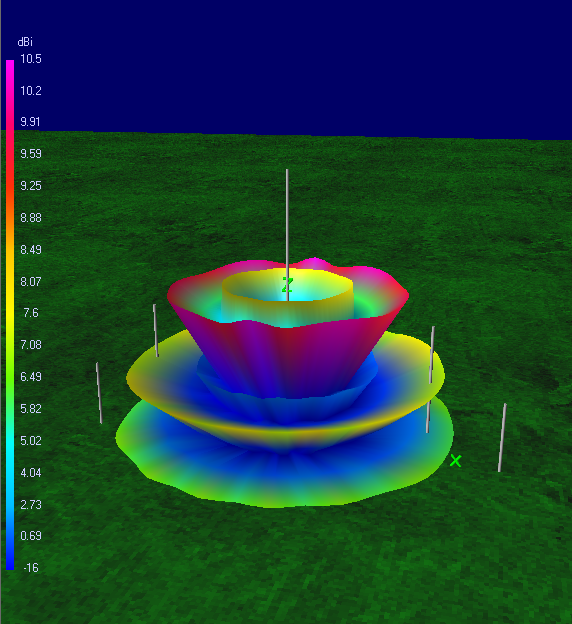
\includegraphics[scale=0.43]{imagenes/3D_480MHz_tierra.png}
	\end{subfigure}
	\caption{$f=\SI{480}{\mega\hertz}$.}
	\label{fig.radiacion_480M_tierra}
\end{figure}	

%%%%%%%%%% 4. CORRIENTES %%%%%%%%%%
\begin{figure}[H]
	\begin{subfigure}{0.5\textwidth}
		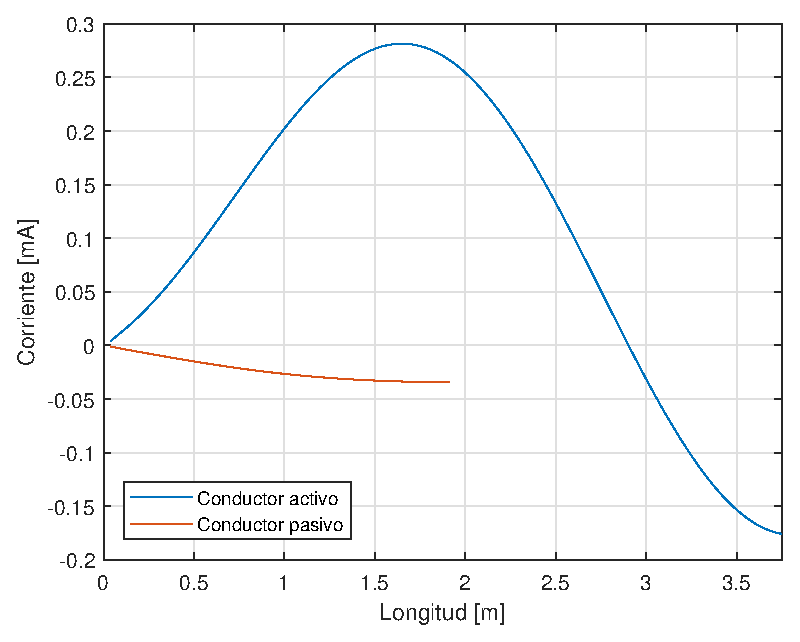
\includegraphics[scale=0.6]{imagenes/i_real_80_tierra.eps}
		\caption{Parte real.}
	\end{subfigure}
	\quad
	\begin{subfigure}{0.5\textwidth}
		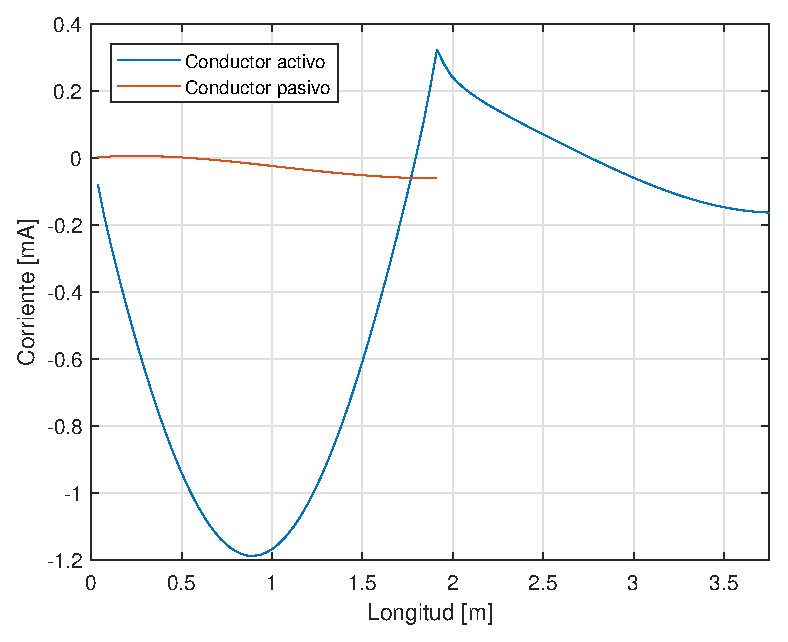
\includegraphics[scale=0.6]{imagenes/i_imag_80_tierra.eps}
		\caption{Parte imaginaria.}
	\end{subfigure}
	\quad
	\begin{subfigure}{0.5\textwidth}
		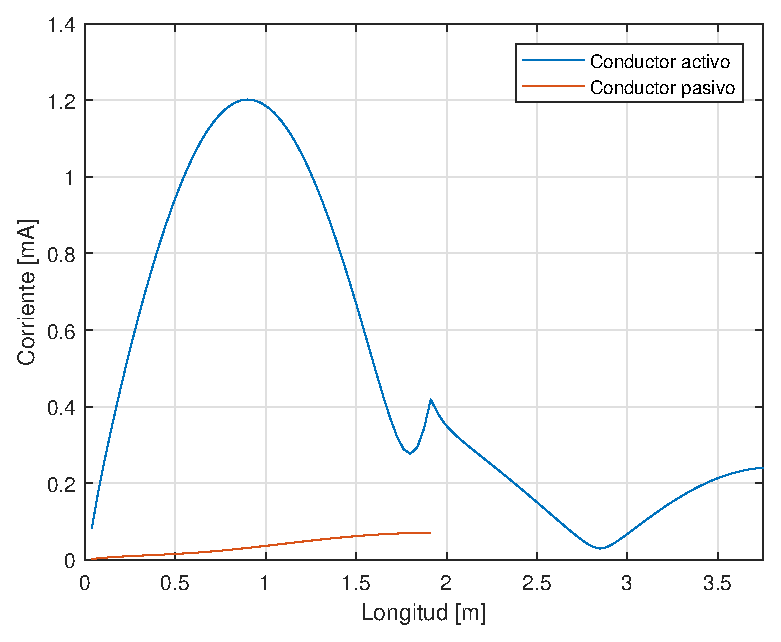
\includegraphics[scale=0.6]{imagenes/i_mag_80_tierra.eps}
		\caption{Magnitud.}
	\end{subfigure}
	\quad
	\begin{subfigure}{0.5\textwidth}
		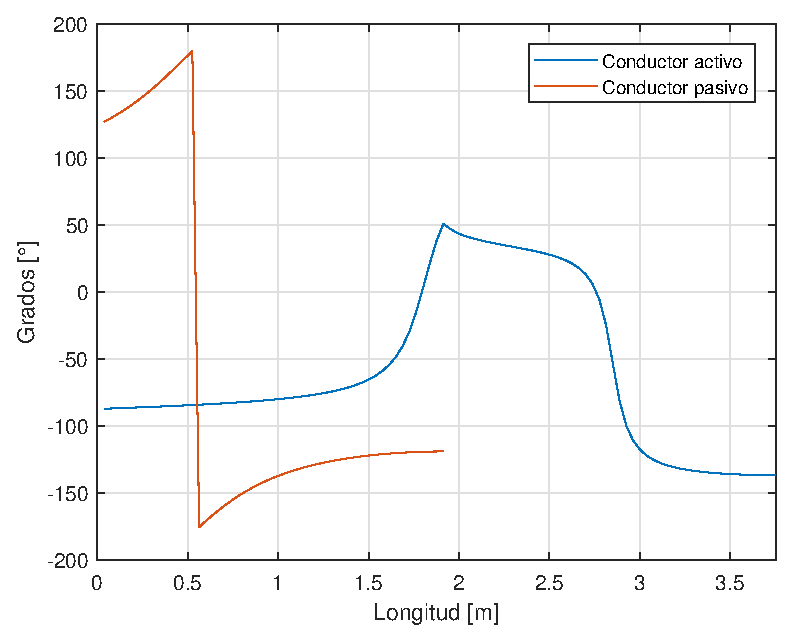
\includegraphics[scale=0.6]{imagenes/i_fase_80_tierra.eps}
		\caption{Fase.}
	\end{subfigure}
	\caption{Corriente para la frecuencia mínima $f = \SI{80}{\mega\hertz}$}
\end{figure}


\begin{figure}[H]
	\begin{subfigure}{0.5\textwidth}
		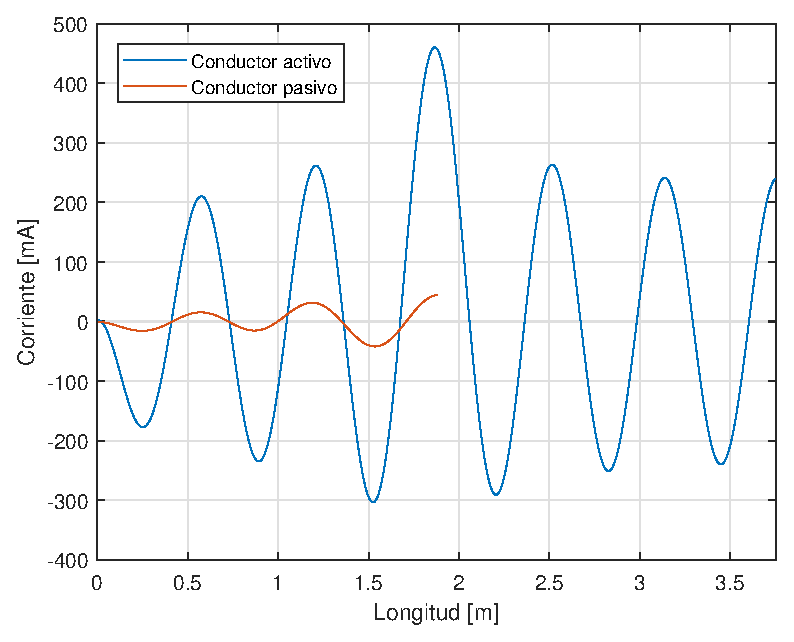
\includegraphics[scale=0.6]{imagenes/i_real_480_tierra.eps}
		\caption{Parte real.}
	\end{subfigure}
	\quad
	\begin{subfigure}{0.5\textwidth}
		\includegraphics[scale=0.6]{imagenes/i_imag_480_tierra.eps}
		\caption{Parte imaginaria.}
	\end{subfigure}
	\quad
	\begin{subfigure}{0.5\textwidth}
		\includegraphics[scale=0.6]{imagenes/i_mag_480_tierra.eps}
		\caption{Magnitud.}
	\end{subfigure}
	\quad
	\begin{subfigure}{0.5\textwidth}
		\includegraphics[scale=0.6]{imagenes/i_fase_480_tierra.eps}
		\caption{Fase.}
	\end{subfigure}
	\caption{Corriente para la frecuencia máxima $f = \SI{480}{\mega\hertz}$}
\end{figure}		
	\pagebreak					
	\section{Conclusiones}
		En base a las simulaciones realizadas se logró determinar la radiación emitida por cierta configuración, resultando un correcto funcionamiento sólo para algunas frecuencias debido a la aparición de lóbulos secundarios capaces de desviar la directividad de la antena.
		
	%\appendix
\end{document}
